\subsection{Interpretable Models} \label{sec:interp_models}
\citet{Doshi-Velez2017-xy} give an argument for why interpretability is critical in AIA systems when they say that interpretability `is used to confirm other important desiderata of ML systems'. They use the words `interpretable' and `explainable' interchangeably. In contrast we treat them as distinct topics. Interpretable models, are defined here as those models that are intrinsically interpretable, and are \emph{integral} to the AIA. This is opposed to `explainable' models which are discussed in Section~\ref{sec:reduce_complexity}, and are \emph{supplemental} to the AIA. A model might be both interpretable \emph{and} explainable, but this is not necessarily the case.

\subsubsection{Common Approaches:}
typically focus on evaluating what models are interpretable via human trials. models based on human intuition

\paragraph{Which Models Are Inherently Interpretable:}
\citet{Van_Belle2013-ph} suggested three ways to ascertain the level of interpretability and potential utility of learned models (compare to categories proposed by \citet{Lipton2016-ug}): 1) Map them to domain knowledge; 2) Ensure safe operation across the full operational range of model inputs; and 3) Assess whether important non-linear effects are accurately accounted for. This work identifies certain strengths and weaknesses of different techniques, but ultimately concludes that no method is clearly best in all situations.

Along similar lines, \citet{Huysmans2011-th} compared decision trees, decision tables, propositional if-then rules, and oblique rule sets to understand which set of methods is `most interpretable'. It was experimentally determined that decision trees and tables tend to be easier to interpret, but it is noted that each method could perform better than others in different applications. For example decision trees and tables are typically better suited for answering a symbolic question (which requires a local understanding of a model) like: \emph{how does the model classify observation $X$'?} ; This is in contrast to a spatial question (which requires a global understanding of the model) like: \emph{is it correct that applicants with a high income are more likely to be accepted than applicants with a low income?}
%%%%%%%%%%%%%%%%%%%%%%%%%
\begin{figure}[htbp]
    \centering
    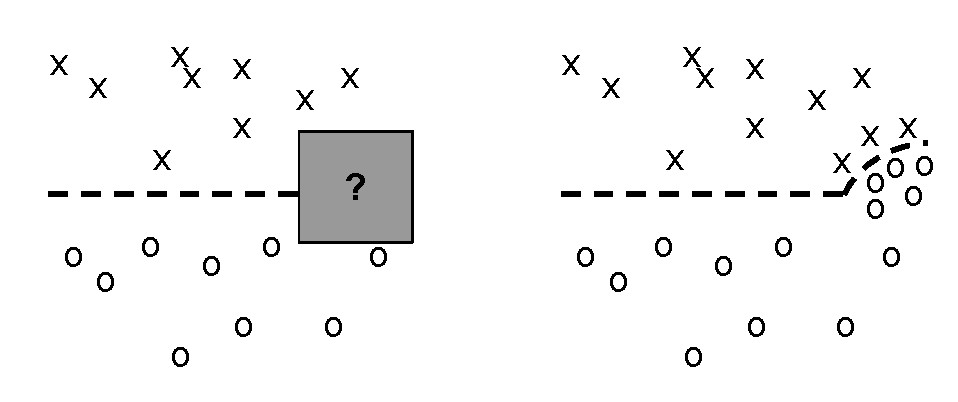
\includegraphics[width=0.5\textwidth]{Figures/global_local}
    \caption{Example of simple global interpretable learning model on the left, and on the right a more complex locally interpretable learning model that can be used when more precise understanding of a specific decision made by the learner is required. }
    \label{fig:ruping}
\end{figure}
%%%%%%%%%%%%%%%%%%%%%%%%%

\paragraph{What Makes An Interpretable Model:}
\citet{Park2016-ld} point out that real interpretability in complex tasks still requires expert knowledge to make sense of complicated features; in essence: \emph{people make interpretable models}. For instance, \citet{Jovanovic2016-gw} use `Tree-Lasso' (TL) logistic regression with domain knowledge (i.e. medical diagnostic codes) to group similar conditions, and then use TL regression again on that information to develop a sparser model. \citet{Zycinski2012-jj} also use domain knowledge to structure a data matrix before feature selection and classification. See also \citet{Zhang2018-no,Khoa2018-gh} for other related examples.

\citet{Kumar2016-yw,Faghmous2014-og} argues that interpretable models are \emph{necessary} in data science when studying scientific phenomena such as environmental effects. They propose using `theory guided data science' (TGDS) to provide theoretically interpretable structures to data science problems. As one example of TGDS, \citet{Morrison2016-fz} address the situation where an imperfect analytical model is available for chemical reaction kinetics: the theoretical reaction equations are well known, but a `stochastic operator' is added on top of this to account for uncertainties and modeling errors.

\citet{Abdollahi2016-vn} investigate making collaborative filtering models more interpretable by using a conditional restricted Boltzmann machine (RBM). \citet{Ridgeway1998-lv} use `weight of evidence' (WoE) as a boosting method that is more amenable to interpretation, and show that WoE is on par with AdaBoost. \citet{Choi2016-by} construct a recursive attention neural network to remove recurrence on the hidden state vector, and instead add recurrence on the visits of patients to doctors, as well as on different diagnoses during those visits. In this way the model is able to predict possible diagnoses in time, and a visualization can be that that indicates the critical visits and diagnoses that lead to that prediction.

Contrary to the belief that interpretable models are necessarily less accurate than their less interpretable counterparts several researchers have shown that this is not always the case. However, the real trade-off is the amount of work that goes in to crafting the interpretable model from the start; these methods are often custom designed for certain tasks and are not easily transferable to other problems. Because of this designers of AIAs must strike a balance between \emph{interpretable models}, \emph{explainable models}, and \emph{black-box models}.

\subsubsection{Grounding Example:}
In the case of the `VIP Escort' problem (described in Section~\ref{sec:mot_example}), interpretable models might be used as an assurance in the following way:

We make the following assumptions

\begin{itemize}
    \item The UGV has just begun an attempt to escape the road-network
    \item The UGV is using a decision-tree for selecting different movements
    \item The operator is able to view the decision-tree model the UGV is using
\end{itemize}

While the operator is monitoring the progress of the UGV in its attempt to escape the road-network they are able to consult the decision-tree model. In this case the operator chose to consult the table when they saw the UGV make an unexpected turn at a given intersection. The operator identified the conditions that led to the decision and found that the UGV was not well equipped to execute the decision the operator thought was best.
\paragraph{\textbf{Discussion of Example:}} In this example the use of a decision-tree as a model enabled the operator to investigate unexpected behavior. During inspection they identified certain conditions that led to a decision, and they found that the UGV was not \emph{competent} to perform what the operator thought was a better decision. Because of this the operator better understood the decision the UGV made.
